\documentclass[11pt,a4paper]{article}
\usepackage[T1]{fontenc}
\usepackage[utf8]{inputenc}
\usepackage{lmodern}
\usepackage[margin=2.3cm]{geometry}
\usepackage{microtype}
\usepackage{amsmath,amssymb,mathtools}
\usepackage{booktabs}
\usepackage{graphicx}
\usepackage[dvipsnames]{xcolor}
\usepackage{tikz}
\usetikzlibrary{arrows.meta,positioning,fit,calc,decorations.pathreplacing}
\usepackage{caption}
\captionsetup{font=small,labelfont=bf}
\usepackage{enumitem}
\setlist{itemsep=2pt,topsep=4pt}
\usepackage{fancyhdr}
\usepackage[hidelinks]{hyperref}

\definecolor{ink}{HTML}{1F2937}
\definecolor{acc}{HTML}{C2410C}
\definecolor{acc2}{HTML}{1D4ED8}
\definecolor{soft}{HTML}{F3F4F6}

\pagestyle{fancy}
\fancyhf{}
\fancyhead[L]{\small Drift --- technical description}
\fancyhead[R]{\small\thepage}
\renewcommand{\headrulewidth}{0.3pt}

\newcommand{\code}[1]{\texttt{#1}}
\DeclareMathOperator{\GELU}{GELU}
\DeclareMathOperator{\clip}{clip}
\newcommand{\E}{\mathbb{E}}
\newcommand{\R}{\mathbb{R}}

\begin{document}

\begin{center}
{\LARGE\bfseries Drift}\\[4pt]
{\large A neural surface-code decoder that adapts to drifting noise\\from its own syndrome statistics}\\[10pt]
{\normalsize Technical description: architecture, data generation, data format, training and evaluation}\\[6pt]
{\small Chahat Patel \quad$\cdot$\quad 8 November 2026}
\end{center}

\vspace{4pt}
\noindent\fbox{\parbox{\dimexpr\linewidth-2\fboxsep-2\fboxrule}{\small
\textbf{Scope.} This document describes the code as it stands after round 4 of experiments
(\code{circuits.py}, \code{drift.py}, \code{make\_dataset.py}, \code{decoder.py}, \code{train.py},
\code{baselines.py}, \code{eval.py}). The data statistics in Section~\ref{sec:data} and the parameter counts in
Section~\ref{sec:arch} were measured from the code, not estimated. Results in Section~\ref{sec:results} come from the
experiment reports; d=5 numbers are from one model seed (seed~0) unless marked.}}

\tableofcontents
\vspace{6pt}

%=====================================================================
\section{What the system does}
%=====================================================================

A quantum memory stores one logical qubit in many physical qubits arranged as a \emph{surface code}.
Errors on the physical qubits are never observed directly. Instead, the hardware repeatedly measures
\emph{stabilisers}, and a \emph{decoder} reads the resulting \emph{detection events} and predicts
whether the logical qubit was flipped.

On real hardware the error rates are not constant: qubits slowly drift, defects switch on and off,
and radiation events briefly corrupt clusters of qubits. A decoder tuned to one noise model gets
worse when the noise moves. Drift is a neural decoder that receives, next to the current shot, a
\emph{fingerprint}: the firing rate of every detector over its own recent shots. It never receives
calibration data or the true noise. The research question is whether this self-supervised signal
lets it keep up with drift better than (a) the same network without the fingerprint and
(b) classical decoders that re-estimate the noise from the same syndrome stream.

\begin{figure}[h]
\centering
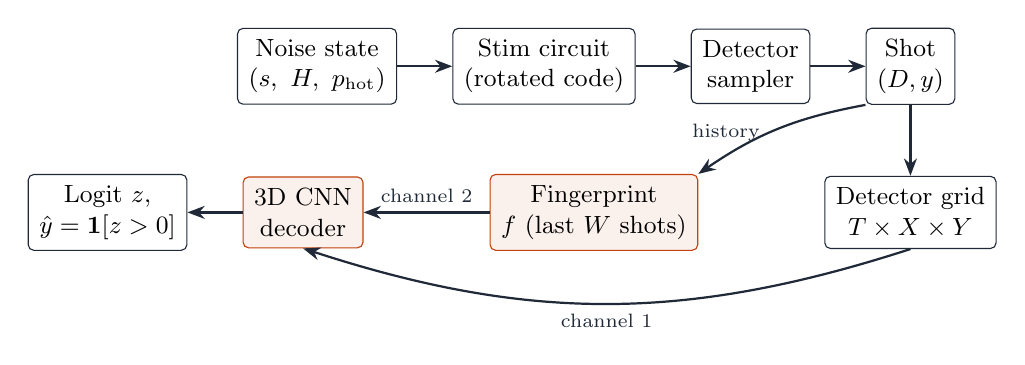
\begin{tikzpicture}[
  box/.style={draw=ink, rounded corners=2pt, align=center, font=\small, minimum height=9mm, inner sep=4pt, fill=white},
  hl/.style={box, fill=acc!8, draw=acc},
  arr/.style={-{Stealth[length=2.2mm]}, thick, ink},
  node distance=6mm and 7mm]
\node[box] (ns) {Noise state\\$(s,\ H,\ p_{\mathrm{hot}})$};
\node[box, right=of ns] (circ) {Stim circuit\\(rotated code)};
\node[box, right=of circ] (samp) {Detector\\sampler};
\node[box, right=of samp] (shot) {Shot\\$(D, y)$};
\node[box, below=9mm of shot] (grid) {Detector grid\\$T\times X\times Y$};
\node[hl, left=16mm of grid] (fp) {Fingerprint\\$f$ (last $W$ shots)};
\node[hl, left=16mm of fp] (net) {3D CNN\\decoder};
\node[box, left=of net] (out) {Logit $z$,\\$\hat y = \mathbf 1[z>0]$};
\draw[arr] (ns) -- (circ);
\draw[arr] (circ) -- (samp);
\draw[arr] (samp) -- (shot);
\draw[arr] (shot) -- (grid);
\draw[arr] (shot.south west) to[bend right=12] node[font=\scriptsize, left, pos=0.55]{history} (fp.north east);
\draw[arr] (grid.south) to[bend left=18] node[font=\scriptsize, below]{channel 1} (net.south);
\draw[arr] (fp) -- node[font=\scriptsize, above]{channel 2} (net);
\draw[arr] (net) -- (out);
\end{tikzpicture}
\caption{Data flow. Stim simulates noisy shots of a surface-code memory experiment. Each shot's
detection events are laid out on a 3D grid; an adaptive decoder also gets the fingerprint, built
from previously seen shots only.}
\label{fig:pipeline}
\end{figure}

%=====================================================================
\section{The code and its detection events}\label{sec:code}
%=====================================================================

\subsection{Memory experiment}
Every shot is a \emph{rotated surface-code memory experiment in the $Z$ basis}, generated by
Stim as \code{surface\_code:rotated\_memory\_z} with code distance $d$ and $r$ rounds of stabiliser
measurement (always $r=d$ in this project). A distance-$d$ rotated code uses $d^2$ data qubits and
$d^2-1$ measure qubits: $(d^2-1)/2$ measure $Z$-type stabilisers and $(d^2-1)/2$ measure $X$-type
stabilisers (Figure~\ref{fig:layout}).

\begin{figure}[h]
\centering
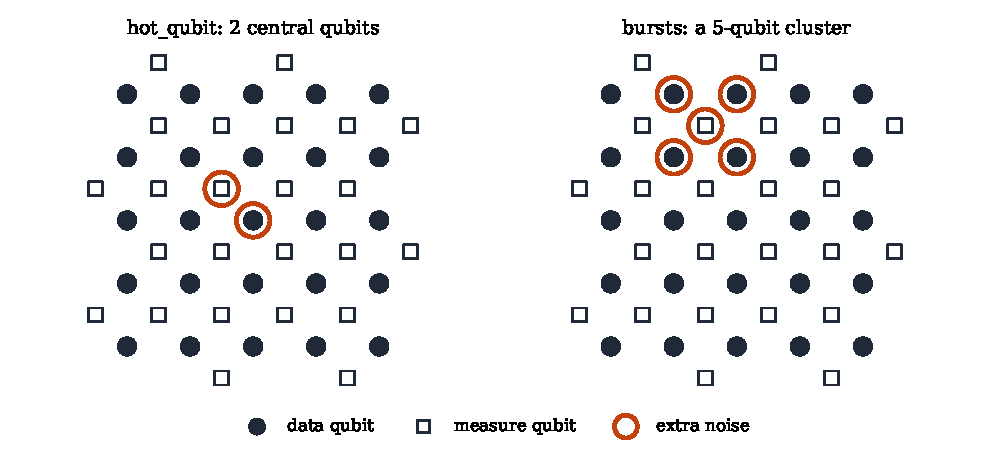
\includegraphics[width=0.88\linewidth]{fig/layout.pdf}
\caption{The $d=5$ patch (25 data qubits, 24 measure qubits) in Stim's coordinates, with the qubits
that receive extra noise in two of the drift regimes. In \code{hot\_qubit} the two qubits closest to the
centre of the patch are chosen; in \code{bursts} a cluster is formed around a random qubit.}
\label{fig:layout}
\end{figure}

\subsection{Detection events}
Let $m_{a,t}\in\{0,1\}$ be the outcome of stabiliser $a$ in round $t$. A \emph{detector} compares
consecutive outcomes, and a \emph{detection event} is a detector that fires:
\begin{equation}
  D_{a,t} = m_{a,t} \oplus m_{a,t-1}.
\end{equation}
Without errors every $D_{a,t}=0$, so a firing detector marks the place and time of an error.
In the first layer only the $Z$-type detectors are deterministic (the data qubits start in $|0\rangle$),
and the last layer compares the final data-qubit measurements with the last $Z$-stabiliser round. Counting
layers gives the number of detectors per shot:
\begin{equation}
  N \;=\; \underbrace{\tfrac{d^2-1}{2}}_{t=0}
  \;+\; \underbrace{(r-1)\,(d^2-1)}_{t=1,\dots,r-1}
  \;+\; \underbrace{\tfrac{d^2-1}{2}}_{t=r}
  \;=\; r\,(d^2-1).
\end{equation}
For $d=r=3$ this is $N=24$; for $d=r=5$ it is $N=120$. Both match Stim.

\subsection{Label}
Each shot has one \emph{observable}: the parity of the final data-qubit measurements along a logical
$Z$ string. The label is
\begin{equation}
  y \in \{0,1\},\qquad y = 1 \iff \text{the logical qubit was flipped.}
\end{equation}
A decoder sees $D\in\{0,1\}^N$ and outputs a prediction $\hat y$. It makes a \emph{logical error}
when $\hat y \neq y$. The logical error rate (LER) is the fraction of shots with a logical error.

%=====================================================================
\section{Noise model and drift}\label{sec:noise}
%=====================================================================

\subsection{Baseline noise}
The nominal circuit uses uniform circuit-level depolarising noise of strength $p_0 = 0.003$ at every
location Stim exposes:
\begin{itemize}
  \item \code{DEPOLARIZE2}$(p)$ after every two-qubit gate,
  \item \code{DEPOLARIZE1}$(p)$ on every data qubit before every round,
  \item \code{X\_ERROR}$(p)$ after every reset,
  \item \code{X\_ERROR}$(p)$ before every measurement.
\end{itemize}
The single-qubit depolarising channel applies a uniformly random non-identity Pauli with probability $p$:
\begin{equation}
  \mathcal{D}_p(\rho) \;=\; (1-p)\,\rho \;+\; \frac{p}{3}\bigl(X\rho X + Y\rho Y + Z\rho Z\bigr).
\end{equation}
The two-qubit channel likewise applies each of the 15 non-identity two-qubit Paulis with probability $p/15$.

\subsection{Noise state}
At any moment the noise is a \emph{noise state} $\mathcal{N} = (s,\, H,\, p_{\mathrm{hot}})$:
\begin{itemize}
  \item a global scale $s>0$, so every location above uses $p = s\,p_0$;
  \item a set $H$ of ``hot'' qubits (possibly empty);
  \item an extra strength $p_{\mathrm{hot}}$: after every \code{TICK} (every circuit layer), each hot qubit
        receives an additional $\mathcal{D}_{p_{\mathrm{hot}}}$.
\end{itemize}
The state $(1,\varnothing,0)$ is called \emph{nominal}. So that circuits can be cached, the scale is
rounded before a circuit is built: $\hat s = \max\bigl(0.05,\ 0.05\cdot\mathrm{round}(s/0.05)\bigr)$.
Hot qubits are always chosen as the $k$ qubits nearest (in Stim's coordinates) to some centre,
which makes them a spatially correlated cluster, as a radiation event or a defect would be.

\subsection{Drift regimes}
Time is divided into \emph{steps}. Within a step the noise state is fixed and $2000$ shots are sampled;
between steps it evolves by one of the regimes below (Figure~\ref{fig:regimes}). Streams are $150$ steps long.

\begin{description}[leftmargin=1.2em, labelindent=0em]
\item[\code{static}] $\mathcal N_t = (1,\varnothing,0)$ for every $t$. Control.
\item[\code{wander}] Slow drift of the global scale: an Ornstein--Uhlenbeck walk in $\log s$,
  \begin{equation}
    x_{t+1} = \clip\!\bigl(x_t - \theta x_t + \sigma\,\varepsilon_t,\ \ln 0.5,\ \ln 2.5\bigr),\quad
    \varepsilon_t\sim\mathcal N(0,1),\quad s_t = e^{x_t},
  \end{equation}
  with $\theta=0.03$, $\sigma=0.08$, $x_0=0$.
\item[\code{telegraph}] Random telegraph noise: $s_t\in\{1,2\}$, and at each step the level switches with
  probability $0.04$.
\item[\code{hot\_qubit}] A persistent local change: from step $\lfloor T/3\rfloor$ on, the two qubits nearest the
  centre are hot with $p_{\mathrm{hot}} = 0.03$.
\item[\code{bursts}] Radiation-like events: when no burst is active, a burst starts with probability $0.04$;
  it picks a random centre qubit, makes the $5$ qubits nearest to it hot with $p_{\mathrm{hot}}=0.05$, and
  lasts $4$ steps.
\item[\code{bursts\_big}] \emph{Held-out test regime}: as \code{bursts} but with $8$-qubit clusters and
  $p_{\mathrm{hot}}=0.1$, outside the training range (Section~\ref{sec:traindist}).
\end{description}

\begin{figure}[h]
\centering
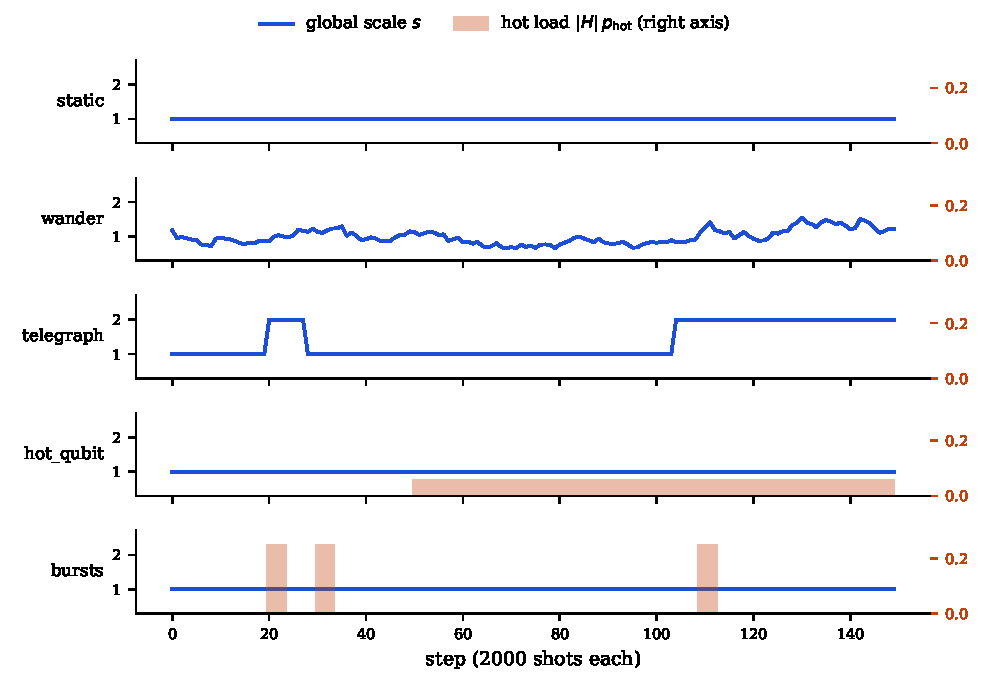
\includegraphics[width=0.86\linewidth]{fig/regimes.pdf}
\caption{One sample schedule of each regime ($d=5$, 150 steps). Blue: global scale $s_t$ (left axis).
Orange: hot load $|H|\,p_{\mathrm{hot}}$ (right axis).}
\label{fig:regimes}
\end{figure}

\subsection{Training noise distribution}\label{sec:traindist}
Training never uses the regimes. Each training \emph{chunk} draws an independent noise state:
\begin{align}
  \ln s &\sim \mathcal U\bigl(\ln 0.5,\ \ln 2.5\bigr), \\
  \text{with prob. } \tfrac12:\qquad
  k &\sim \mathcal U\{1,\dots,6\},\quad c \sim \mathcal U(\text{all qubits}),\quad
  p_{\mathrm{hot}} \sim \mathcal U(0.005,\ 0.08), \notag\\
  H &= \text{the } k \text{ qubits nearest to } c, \\
  \text{otherwise}:\qquad H &= \varnothing,\quad p_{\mathrm{hot}} = 0 .
\end{align}
This is the ``wide'' range used since round~2 (the first datasets used $k\le 4$ and $p_{\mathrm{hot}}\le0.05$).
A \emph{nominal-only} dataset fixes every chunk to $(1,\varnothing,0)$; it trains the specialist baseline.
\code{bursts} ($k=5$, $p_{\mathrm{hot}}=0.05$) lies inside the wide range; \code{bursts\_big}
($k=8$, $p_{\mathrm{hot}}=0.1$) lies outside it on both axes.

%=====================================================================
\section{What the data looks like}\label{sec:data}
%=====================================================================

\subsection{One shot as a 3D image}
Every detector has Stim coordinates $(x,y,t)$. Sorting the distinct values on each axis gives a grid of
shape
\begin{equation}
  (T,\,X,\,Y) = (r+1,\ d+1,\ d+1),
\end{equation}
that is $(4,4,4)$ for $d=3$ and $(6,6,6)$ for $d=5$. A shot $D\in\{0,1\}^N$ is written into this grid;
cells without a detector stay $0$. With $\iota_x,\iota_y,\iota_t$ the index of a detector on each axis, its
position in the flattened grid is
\begin{equation}
  \mathrm{flat}(a) = (\iota_t\,X + \iota_x)\,Y + \iota_y .
\end{equation}
Only $N/(TXY)$ of the cells hold a detector: $24/64 = 37.5\%$ at $d=3$ and $120/216 \approx 55.6\%$ at $d=5$.
Figure~\ref{fig:shot} shows two real $d=5$ shots.

\begin{figure}[h]
\centering
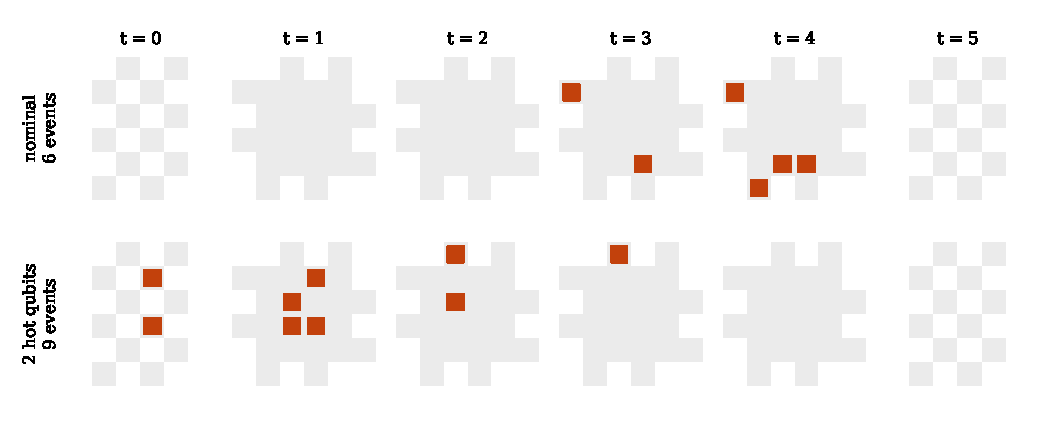
\includegraphics[width=\linewidth]{fig/shot.pdf}
\caption{Two $d=5$ shots on the $6\times6\times6$ grid, one panel per time layer. Grey cells hold a
detector; orange cells fired. Layers $t=0$ and $t=5$ hold only the $Z$-type detectors (checkerboard).
Top: nominal noise. Bottom: the two central qubits are hot, and events cluster around them.}
\label{fig:shot}
\end{figure}

\subsection{Statistics}
Table~\ref{tab:stats} gives measured statistics from $10^5$ nominal shots. Detection events are sparse:
at $d=5$ about $4.3\%$ of detectors fire, about five per shot. The raw observable flip rate is what a
decoder that always answers ``no flip'' would score; a decoder has to bring it down to the LER
(about $0.0033$ for MWPM at $d=5$).

\begin{table}[h]
\centering
\small
\begin{tabular}{lrr}
\toprule
 & $d=r=3$ & $d=r=5$ \\
\midrule
Physical qubits (data + measure) & $9 + 8 = 17$ & $25 + 24 = 49$ \\
Detectors per shot $N = r(d^2-1)$ & $24$ & $120$ \\
Grid $(T,X,Y)$ & $(4,4,4)$ & $(6,6,6)$ \\
Grid cells holding a detector & $37.5\%$ & $55.6\%$ \\
Mean detector firing rate (nominal) & $3.61\%$ & $4.27\%$ \\
Detection events per shot (nominal) & $0.87$ & $5.12$ \\
Shots with at least one event & $40.3\%$ & $92.3\%$ \\
Raw observable flip rate $\Pr[y=1]$ & $6.57\%$ & $15.36\%$ \\
\bottomrule
\end{tabular}
\caption{Measured statistics of nominal shots ($p_0 = 0.003$, $10^5$ shots).}
\label{tab:stats}
\end{table}

\noindent Drift changes these numbers. At $d=5$ the mean number of events per shot is $5.15$ (nominal),
$9.84$ (scale $\times2$), $8.30$ (two hot qubits, $p_{\mathrm{hot}}=0.03$) and $14.28$ (a five-qubit burst,
$p_{\mathrm{hot}}=0.05$), measured over $5\times10^4$ shots each.

\subsection{The fingerprint}
The fingerprint is the empirical firing rate of each detector over the last $W$ shots the decoder has
seen ($W=2000$):
\begin{equation}
  f_a \;=\; \frac{1}{W}\sum_{k=1}^{W} D^{(k)}_a ,\qquad f\in[0,1]^N .
\end{equation}
It is laid out on the same grid as the shot and multiplied by $10$, so its values sit in a range similar
to the $0/1$ events. Since $f_a$ estimates $\Pr[D_a = 1]$, it reflects both the overall noise level and
where the noise is concentrated (Figure~\ref{fig:fp}). With $W=2000$ shots, the binomial standard error of
one rate near $0.043$ is $\sqrt{0.043\cdot 0.957/2000}\approx 0.0045$, about $10\%$ of the rate.

\begin{figure}[h]
\centering
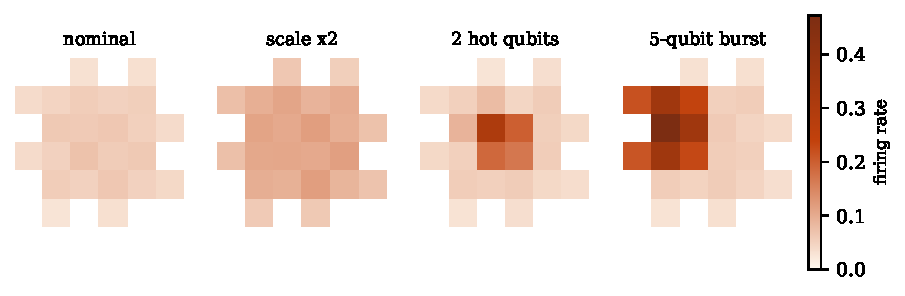
\includegraphics[width=0.95\linewidth]{fig/fingerprint.pdf}
\caption{Fingerprints at $d=5$ ($W=2000$ shots), averaged over the four middle time layers.
A global scale change raises every rate; hot qubits and bursts raise the rates of nearby detectors only.}
\label{fig:fp}
\end{figure}

\subsection{Datasets on disk}
\code{make\_dataset.py} writes a folder \code{data/<name>/} with a \code{manifest.json} that records the
generation arguments, the seed of every split, library versions, array shapes and the SHA-256 of every file.
Every split gets its own seed derived from the main seed,
\begin{equation*}
  \mathrm{seed}_{\text{split}} = \mathrm{SeedSequence}\bigl(\mathrm{seed},\ \mathrm{crc32}(\text{split name})\bigr),
\end{equation*}
so train, validation, test and stream shots are independent samples. All arrays are bit-packed
(\code{np.packbits}) and stored as compressed \code{.npz}.

\begin{description}[leftmargin=1.2em, labelindent=0em]
\item[Training chunks] (\code{train.npz}, \code{val.npz}). A \emph{chunk} is one noise state drawn as in
  Section~\ref{sec:traindist}, plus $B=512$ training shots and, for adaptive models, $W=2000$ further
  shots from the \emph{same} noise used only for the fingerprint. Arrays: \code{det} (chunks, $512$, $\lceil N/8\rceil$ bytes),
  \code{obs} (labels, packed along the shot axis), \code{window\_det} (chunks, $2000$, $\lceil N/8\rceil$),
  and the noise state of each chunk. At $d=5$ one chunk is about $37.7$\,kB before compression,
  $80\%$ of it fingerprint shots.
\item[Test sets] (\code{test\_*.npz}). Three fixed states: nominal; scale $\times2$; two central hot qubits
  with $p_{\mathrm{hot}}=0.03$. Each has $200\,000$ shots plus $2000$ fingerprint shots.
\item[Streams] (\code{stream\_<regime>[\_seed<n>].npz}). The noise state of every step and
  $150\times2000$ shots. Stream seeds $0$--$4$ give five independent streams per regime.
\end{description}

\begin{table}[h]
\centering
\small
\begin{tabular}{llrrr}
\toprule
Dataset & Training noise & Train chunks & Train shots & On disk \\
\midrule
\code{d3\_wide} & wide & $30\,000$ & $15.4$\,M & $\approx0.1$\,GB \\
\code{d5\_wide} & wide & $30\,000$ & $15.4$\,M & $510$\,MB \\
\code{d5\_nominal} & nominal only & $30\,000$ & $15.4$\,M & $86$\,MB \\
\code{d5\_wide\_x5} & wide & $150\,000$ & $76.8$\,M & $2.3$\,GB \\
\code{d5\_nominal\_x5} & nominal only & $150\,000$ & $76.8$\,M & $393$\,MB \\
\bottomrule
\end{tabular}
\caption{Datasets used so far. All have $1000$ validation chunks. Nominal-only sets store no fingerprint
shots (\code{-{}-window 0}), which is why they are much smaller. Test sets and streams are byte-identical
across datasets made with the same seed.}
\label{tab:datasets}
\end{table}

Stim only guarantees identical samples for a seed on the same Stim version and machine, which is why the
data is saved rather than regenerated. All runs so far used Stim 1.16.0, PyMatching 2.4.0, NumPy 2.4.6 and
PyTorch 2.15.0.

%=====================================================================
\section{Decoder architecture}\label{sec:arch}
%=====================================================================

\subsection{Network}
The decoder (\code{ConvDecoder} in \code{decoder.py}) is a small 3D convolutional network. Its input is
$x\in\R^{C\times T\times X\times Y}$ with $C=1$ (static: the shot) or $C=2$ (adaptive: shot and fingerprint).
With $L$ layers of width $H$:
\begin{align}
  h^{(0)} &= x, \\
  h^{(\ell)} &= \GELU\bigl(K^{(\ell)} * h^{(\ell-1)} + b^{(\ell)}\bigr), \qquad \ell = 1,\dots,L,
\end{align}
where $K^{(\ell)}$ is a $3\times3\times3$ convolution with zero padding $1$ (the grid size is kept) and
$H$ output channels. The last feature map is pooled over all $TXY$ positions, by mean and by maximum, and
the two are concatenated:
\begin{equation}
  u = \Bigl[\ \tfrac{1}{TXY}\sum_{v} h^{(L)}_{:,v}\ \ ;\ \ \max_{v} h^{(L)}_{:,v}\ \Bigr] \in \R^{2H}.
\end{equation}
A two-layer head produces one logit:
\begin{equation}
  z = w_2^{\top}\,\GELU\bigl(W_1 u + b_1\bigr) + b_2,\qquad W_1\in\R^{64\times 2H},\ w_2\in\R^{64}.
\end{equation}
The predicted probability of a logical flip is $\sigma(z) = 1/(1+e^{-z})$, and the decision is
$\hat y = \mathbf 1[z>0]$.

\begin{figure}[h]
\centering
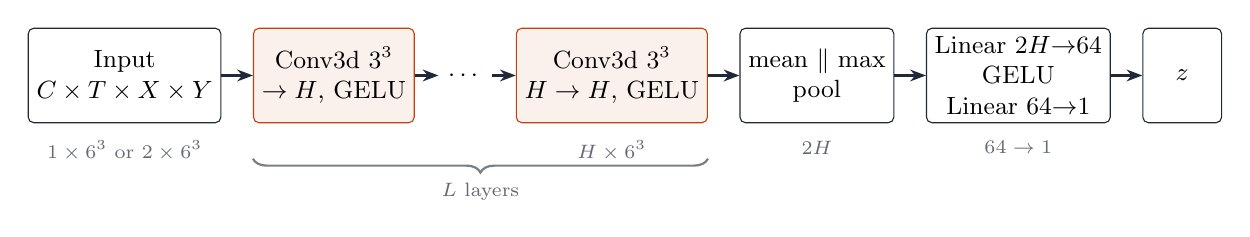
\begin{tikzpicture}[
  lay/.style={draw=ink, rounded corners=2pt, align=center, font=\small, minimum height=12mm, minimum width=18mm, fill=white, inner sep=3pt},
  hl/.style={lay, fill=acc!8, draw=acc},
  arr/.style={-{Stealth[length=2mm]}, thick, ink},
  dim/.style={font=\scriptsize, text=ink!70},
  node distance=4mm]
\node[lay] (in) {Input\\$C\times T\times X\times Y$};
\node[hl, right=of in] (c1) {Conv3d $3^3$\\$\to H$, GELU};
\node[font=\small, right=3mm of c1] (dots) {$\cdots$};
\node[hl, right=3mm of dots] (cL) {Conv3d $3^3$\\$H\to H$, GELU};
\node[lay, right=of cL] (pool) {mean $\Vert$ max\\pool};
\node[lay, right=of pool] (head) {Linear $2H{\to}64$\\GELU\\Linear $64{\to}1$};
\node[lay, right=of head, minimum width=10mm] (z) {$z$};
\draw[arr] (in) -- (c1); \draw[arr] (c1) -- (dots); \draw[arr] (dots) -- (cL);
\draw[arr] (cL) -- (pool); \draw[arr] (pool) -- (head); \draw[arr] (head) -- (z);
\node[dim, below=1mm of in] {$1\times6^3$ or $2\times6^3$};
\node[dim, below=1mm of cL] {$H\times6^3$};
\node[dim, below=1mm of pool] {$2H$};
\node[dim, below=1mm of head] {$64 \to 1$};
\draw[decorate, decoration={brace, amplitude=5pt, mirror}, thick, ink!60]
  ($(c1.south west)+(0,-0.45)$) -- node[dim, below=5pt]{$L$ layers} ($(cL.south east)+(0,-0.45)$);
\end{tikzpicture}
\caption{The decoder. Shapes are for $d=5$. Default $H=48$, $L=4$.}
\label{fig:arch}
\end{figure}

\subsection{Size}
Counting weights and biases, the number of parameters is
\begin{equation}
  P(C,H,L) = \underbrace{(27C + 1)\,H}_{\text{first conv}}
  + \underbrace{(L-1)(27H+1)\,H}_{\text{other convs}}
  + \underbrace{(2H+1)\cdot 64}_{\text{head layer 1}}
  + \underbrace{65}_{\text{head layer 2}}
\end{equation}

\begin{table}[h]
\centering
\small
\begin{tabular}{lrr}
\toprule
Configuration & Static ($C=1$) & Adaptive ($C=2$) \\
\midrule
$H=48$, $L=4$ (default) & $194\,385$ & $195\,681$ \\
$H=64$, $L=6$ (capacity check) & $563\,393$ & $565\,121$ \\
\bottomrule
\end{tabular}
\caption{Parameter counts from the formula, matching what \code{train.py} prints. The fingerprint adds
only the $27H$ weights of the extra input channel.}
\end{table}

\noindent Each $3^3$ convolution widens the receptive field by $2$ along every axis, so after $L$ layers
it is $(1+2L)^3$. For $L=4$ that is $9^3$, already larger than the whole $6\times6\times6$ grid, so every
output position can see every detector at $d=5$.

\subsection{Why this design}
The network has no knowledge of the code built in except the grid layout. It treats decoding as
classification of a sparse 3D image. The fingerprint enters as a second image channel, so the same
convolutions can compare ``what fired in this shot'' with ``how often it usually fires here''. The
decoder never sees the noise state; it only sees statistics of shots it has already decoded.

%=====================================================================
\section{Training}\label{sec:training}
%=====================================================================

\subsection{Objective and optimiser}
Each step uses one chunk: its $B=512$ shots and (adaptive) the fingerprint of its $W=2000$ window shots.
The loss is the mean binary cross-entropy of the logits:
\begin{equation}
  \mathcal L = -\frac{1}{B}\sum_{i=1}^{B}\Bigl[\,y_i\log\sigma(z_i) + (1-y_i)\log\bigl(1-\sigma(z_i)\bigr)\Bigr].
\end{equation}
Optimisation uses AdamW with peak learning rate $10^{-3}$ and PyTorch's OneCycle schedule over the whole run
(other settings are PyTorch defaults), fp32, batch $512$. Chunk order is reshuffled every epoch. The
validation loss on the $1000$ validation chunks is logged during training.

\begin{table}[h]
\centering
\small
\begin{tabular}{llll}
\toprule
Round & Data & Steps & Epochs \\
\midrule
d=3 (reports 1--2) & \code{d3\_wide} & $60\,000$ & $2$ \\
d=5 (report 3) & \code{d5\_wide} / \code{d5\_nominal} & $60\,000$ & $2$ \\
d=5 (round 4) & \code{d5\_wide\_x5} / \code{d5\_nominal\_x5} & $300\,000$ & $2$ \\
\bottomrule
\end{tabular}
\caption{Training budgets. Round 4 used $5\times$ more steps on a $5\times$ larger dataset, so each chunk
is still seen twice.}
\end{table}

\subsection{Model variants}
\begin{description}[leftmargin=1.2em, labelindent=0em]
\item[static-nominal] $C=1$, trained on nominal noise only. A specialist for undrifted noise.
\item[static-wide] $C=1$, trained on the wide distribution. Has to cope with drift without information about it.
\item[adaptive-wide] $C=2$, wide distribution, the fingerprint always matches the shots.
\item[adaptive-stale] As adaptive-wide, with stale-fingerprint augmentation (below).
\end{description}
Comparing static-wide with adaptive-wide isolates the value of the fingerprint, since both see the same
chunks in the same order.

\subsection{Stale-fingerprint augmentation}
In training the fingerprint always matched the shots, so the first adaptive models trusted it completely
and decoded badly in the first step of a burst, when the fingerprint still described the old noise.
With probability $q=0.3$ per step (\code{-{}-stale-prob 0.3}) the fingerprint is replaced:
\begin{itemize}
  \item with probability $\tfrac12$, by the fingerprint of another random chunk $j$ (fully stale);
  \item otherwise, by the rates of a mixed window: the first $k$ rows of chunk $j$'s window followed by
        the last $W-k$ rows of this chunk's window, with $k = \lfloor U\cdot W\rfloor$, $U\sim\mathcal U(0,1)$.
        This mimics a window caught mid-transition:
        \begin{equation}
          f^{\mathrm{mix}}_a = \frac{1}{W}\Bigl(\sum_{n=1}^{k} D^{(j,n)}_a + \sum_{n=k+1}^{W} D^{(i,n)}_a\Bigr).
        \end{equation}
\end{itemize}
The augmentation uses its own random generator, so the chunk order is the same with or without it.

\subsection{Engineering}
With a saved dataset, all chunks are copied to the GPU once in bit-packed form. Unpacking, the fingerprint
and the grid layout then run on the GPU, giving exactly the same inputs as the original CPU path. Checkpoints
can be saved every $k$ steps together with optimiser and RNG state, so runs can be resumed.

%=====================================================================
\section{Baselines}\label{sec:baselines}
%=====================================================================

All baselines use minimum-weight perfect matching (MWPM, PyMatching~2.4) on the matching graph of Stim's
detector error model. An edge $e$ with error probability $p_e$ gets the weight
\begin{equation}
  w_e = \ln\frac{1-p_e}{p_e}.
\end{equation}
\begin{description}[leftmargin=1.2em, labelindent=0em]
\item[Static MWPM] Weights from the nominal circuit, never updated.
\item[Oracle MWPM] Weights rebuilt from the \emph{true} noise state at every step. It is not an optimal
  decoder (the neural models beat it on nominal noise), but it is MWPM with perfect knowledge of the noise.
\item[WindowDEM] MWPM re-weighted from the last $w$ shots, with no knowledge of the noise state. This is
  the strongest syndrome-only classical baseline. For an edge between detectors $i$ and $j$, with
  $\langle\cdot\rangle$ the mean over the window, its probability is estimated from how often the two
  detectors fire together:
  \begin{equation}
    \hat p_{ij} = \frac12 - \frac12\sqrt{\,1 - \frac{4\bigl(\langle x_ix_j\rangle - \langle x_i\rangle\langle x_j\rangle\bigr)}
    {1 - 2\langle x_i\rangle - 2\langle x_j\rangle + 4\langle x_ix_j\rangle}\,}.
  \end{equation}
  A detector fires when an odd number of its edges flipped, so
  $1 - 2\langle x_i\rangle = (1-2\hat p_{i\partial})\prod_{j}(1-2\hat p_{ij})$, which gives the boundary edge:
  \begin{equation}
    \hat p_{i\partial} = \frac12\Bigl(1 - \frac{1-2\langle x_i\rangle}{\prod_{j}(1-2\hat p_{ij})}\Bigr).
  \end{equation}
  All estimates are clipped to $[10^{-6},\,0.45]$. Window lengths $w\in\{500,1000,2000,5000,10000\}$ are all
  evaluated, and the best one per regime and phase is reported (chosen after the fact, which flatters WindowDEM).
\end{description}

%=====================================================================
\section{Evaluation protocol}\label{sec:eval}
%=====================================================================

\subsection{Causal streaming}
Every decoder sees the same stream. Each step's $2000$ shots are processed in sub-batches of $200$
(\code{-{}-update-every 200}): a sub-batch is first decoded, and only then added to the decoder's history.
A decoder therefore never adapts to shots it is about to decode.

\subsection{Phases}
Each step is classified by its noise state:
\emph{onset} (the first off-nominal step after a nominal one),
\emph{later} (the other off-nominal steps),
\emph{after} (the first nominal step after an off-nominal one),
\emph{nominal} (all nominal steps), and
\emph{drift} (onset and later together). LERs are pooled over shots: total errors divided by total shots.

\subsection{Frozen-fingerprint control}
An adaptive model is also run with its fingerprint fixed to the nominal one. The live-minus-frozen difference
measures how much of its accuracy comes from adaptation, as opposed to being a better decoder.

\subsection{Statistics}
For an LER $p$ over $n$ shots, the standard error is $\mathrm{SE} = \sqrt{p(1-p)/n}$.
Two decoders are called tied if
\begin{equation}
  |p_a - p_b| < 2\sqrt{\mathrm{SE}_a^2 + \mathrm{SE}_b^2}.
\end{equation}
Because all decoders see the same shots, the main test is the exact paired McNemar test. With $b$ the number of
shots that only decoder~A gets wrong and $c$ the number only decoder~B gets wrong,
\begin{equation}
  p_{\text{McNemar}} = \min\Bigl(1,\ 2\sum_{i=0}^{\min(b,c)}\binom{b+c}{i}\,2^{-(b+c)}\Bigr).
\end{equation}
No multiple-testing correction is applied, so $0.001 < p < 0.05$ is treated as weak evidence.

%=====================================================================
\section{Results so far}\label{sec:results}
%=====================================================================

\subsection{$d=3$ (reports 1--2; 3 model seeds, 5 streams)}
\begin{itemize}
  \item On bursts, the live fingerprint beats the frozen one by a wide margin
        ($0.0725$ vs $0.1311$ drift LER, $p<10^{-300}$): the gain is adaptation.
  \item On nominal noise, adaptive-wide ties the nominal specialist ($0.00532$ vs $0.00536$, $p=0.4$),
        while static-wide pays a $13\%$ hedging cost.
  \item Adaptive models beat the best WindowDEM in every phase of every regime.
  \item On telegraph (uniform drift) live and frozen tie: uniform drift needs no adaptation.
\end{itemize}

\subsection{$d=5$ after longer training (round 4; seed 0; 5 streams)}

\begin{figure}[h]
\centering
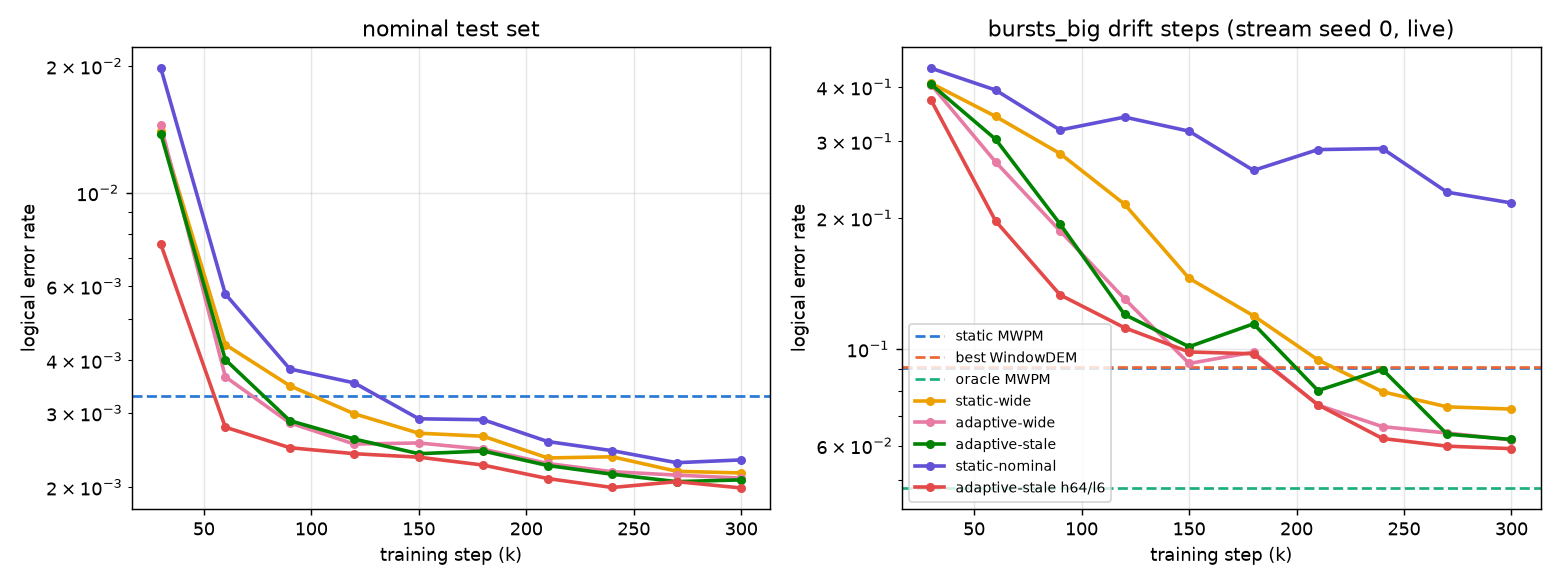
\includegraphics[width=\linewidth]{fig/curves.png}
\caption{Learning curves at $d=5$ (seed 0). Left: nominal test set. Right: \code{bursts\_big} drift steps
(stream seed 0, live fingerprint). Dashed: static MWPM, best WindowDEM, oracle MWPM.}
\label{fig:curves}
\end{figure}

\begin{table}[h]
\centering
\small
\begin{tabular}{lrrrrr}
\toprule
Decoder & nominal test & bursts & bursts\_big & hot\_qubit & telegraph \\
\midrule
Static MWPM & $0.00329$ & $0.0439$ & $0.0980$ & $0.0181$ & $0.0228$ \\
Best WindowDEM & --- & $0.0356$ & $0.0896$ & $0.0108$ & $0.0229$ \\
Oracle MWPM & $0.00329$ & $0.0197$ & $0.0426$ & $0.0103$ & $0.0231$ \\
\midrule
static-nominal & $0.00232$ & $0.0420$ & $0.1596$ & $0.0130$ & $0.0195$ \\
static-wide & $0.00216$ & $0.0241$ & $0.0629$ & $0.0101$ & $0.0184$ \\
adaptive-wide & $0.00210$ & $0.0178$ & $0.0516$ & $0.0074$ & $0.0168$ \\
adaptive-stale & $0.00208$ & $0.0180$ & $0.0514$ & $0.0075$ & $0.0170$ \\
adaptive-stale, $H{=}64$, $L{=}6$ & $0.00199$ & $0.0168$ & $0.0484$ & $0.0070$ & $0.0160$ \\
\bottomrule
\end{tabular}
\caption{$d=5$ LER after $300\,000$ steps (seed 0). Stream columns are drift-step LERs pooled over 5 streams.
Lower is better.}
\label{tab:d5}
\end{table}

\begin{table}[h]
\centering
\small
\begin{tabular}{lrrr}
\toprule
Drift LER, live vs frozen & bursts & bursts\_big & hot\_qubit \\
\midrule
adaptive-wide, live & $0.0178$ & $0.0516$ & $0.0074$ \\
adaptive-wide, frozen & $0.0276$ & $0.0729$ & $0.0107$ \\
adaptive-stale, live & $0.0180$ & $0.0514$ & $0.0075$ \\
adaptive-stale, frozen & $0.0244$ & $0.0639$ & $0.0101$ \\
\bottomrule
\end{tabular}
\caption{The value of the live fingerprint at $d=5$ (seed 0).}
\end{table}

\noindent In summary, at $d=5$ after $300\,000$ steps:
\begin{itemize}
  \item every neural model beats MWPM on nominal noise;
  \item every wide-trained model beats static MWPM and the best WindowDEM on held-out \code{bursts\_big};
  \item the live fingerprint is worth $1$--$2$ points of LER on large bursts;
  \item the adaptive models match or beat oracle MWPM on bursts and hot\_qubit;
  \item a gap to the oracle remains on \code{bursts\_big} ($0.0516$ vs $0.0426$), and the curves were still falling.
\end{itemize}

\subsection{Known limitations}
\begin{itemize}
  \item The $d=5$ round-4 numbers come from one model seed; seeds 1--2 of two models are trained but not yet evaluated.
  \item In the first nominal step after a large burst, the live fingerprint is out of date and adaptive-wide is
        slightly worse than MWPM ($+0.0024$).
  \item Drift regimes use the same absolute cluster sizes at $d=3$ and $d=5$, so absolute LERs are not comparable
        across distances.
  \item Latency (Python, cloud GPU): MWPM is about $5\times$ faster per shot than the neural models at $d=5$.
        This is not a real-time hardware claim.
\end{itemize}

\end{document}
